\documentclass[german,12pt,a4paper]{article}
\usepackage{fullpage}
\usepackage[ngerman]{babel}
\usepackage[utf8]{inputenc}
\usepackage{listings}
\usepackage{verbatim}
\usepackage{enumerate}
\usepackage{graphicx}
\usepackage{float}
\usepackage{wrapfig}
\usepackage{color}
\usepackage[usenames,dvipsnames]{xcolor}
\usepackage[font=small,format=plain,labelfont=bf,up,textfont=it,up]{caption}
\usepackage{subfig}
\usepackage[colorlinks=false, pdfborder={1 0 0}]{hyperref}
\usepackage{qtree}


\pagestyle{plain}
\pagenumbering{arabic}
\frenchspacing

\newcommand{\comments}[1]{}
\renewcommand{\baselinestretch}{1.55}

%Redefine the first level
\renewcommand{\theenumi}{\textbf{\alph{enumi})}}
\renewcommand{\labelenumi}{\theenumi}

\begin{document}

\title{\textbf{Verteilte Systeme SS2012 -- Übung 5}}
\author{Sebastian Menski (734272), Martin Ohmann (734801) \\ \texttt{\{menski,ohmann\}@uni-potsdam.de}}
\date{\today}

\maketitle

\section*{Aufgabe 5.1}

\begin{figure}[h!]
  \centering
  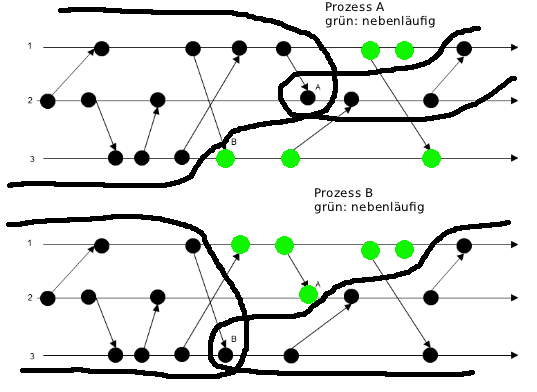
\includegraphics[width=1\textwidth]{aufgabe1.png}
  \caption{Vergangenheits-, Zukunftskegel und Nebenläufigkeit}
\end{figure}

\section*{Aufgabe 5.2}

\begin{enumerate}

	\item Der Zentrale Ansatz bietet eine geringe Fehlertoleranz gegenüber 
	Client- bzw. Server-Crashes. Desweiteren kann der Server bei großer 
	Konkurrenz unter den Sendern zum Flaschenhals werden und das komplette 
	System lahm legen.
	
	\item Das Token-Verfahren ist fehleranfällig, da beim Ausfall eines 
	Prozesses P$_{i}$ / einer Maschine M$_{i}$ ein Tokenverlust erkannt werden 
	muss.
	
	\item Votierungsverfahren

\end{enumerate}

\section*{Aufgabe 5.3}

Durch die eindeutige Weitergabe eines einzigen Tokens wird in einem \glqq{}logischen Ring\grqq{} ein
totale Ordnung definiert.

\section*{Aufgabe 5.4}

\begin{itemize}

	\item Beim Web Service Ring Replication Protocol (WS RRP) wird mit Hilfe des Tokens nicht nur
		der Zugriff geregelt, sondern auch Anwendungs-Nachrichten verteilt. Welche an den Token gehangen
		werden, somit wird keine Multicast-Infrastruktur benötigt.

	\item Beim JGroups-Sequenzer existiert ein extra, zentraler Prozess, welcher eine Ordnung der
		Nachrichten fest. Dies wird per Multicast an die Gruppenmitglieder verteilt, welche sich
		danach an diese Ordnung halten. Dabei basiert das Sequenzer-Protokoll auf den
		pbcast-Protokolle.

	\item Die Response-Zeiten von JGroups sind geringer als von WS RRP. Gründe dafür sind der
		Overhead vom Web-Service-Stack und den GSI-Sicherheits Eigenschaften von WS RRP. So nutzt WS
		RRP für jede Punkt-zu-Punkt Kommunikation einen eigenen Session-Key, hingegegen nutzt
		JGroups eine geteilten Session-Key für das ganze Cluster.

\end{itemize}

\section*{Aufgabe 5.5}

\begin{figure}[h!]
  \centering
  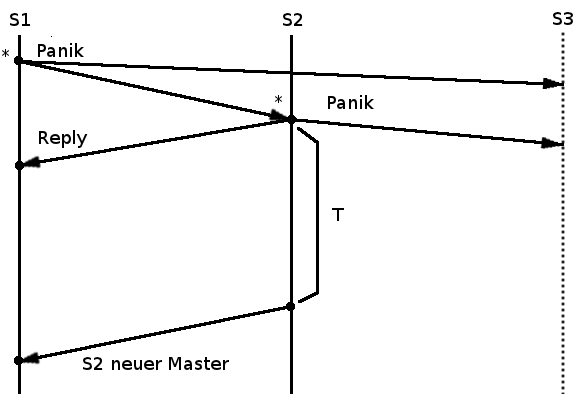
\includegraphics[width=1\textwidth]{bully1.png}
  \caption{Bully-Algorithmus. * Start des Bully-Algorithmus}
\end{figure}

\begin{figure}[h!]
  \centering
  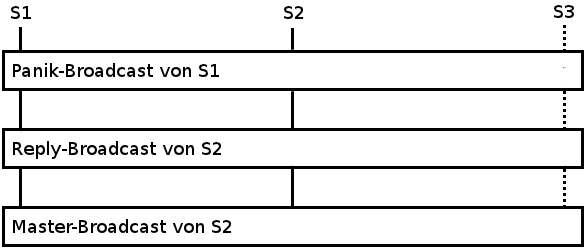
\includegraphics[width=1\textwidth]{bully2.png}
  \caption{Broadcasts im Bully-Algorithmus}
\end{figure}

\end{document}
